\subsection{Task 3.2 -- Deployment diagram}

\subsubsection{Nền tảng triển khai}

Nhóm chọn \textbf{Render} làm nền tảng production vì hỗ trợ Docker Compose-compatible workflow,
PostgreSQL managed không public, HTTPS tự động và tích hợp GitHub Actions qua Render Deploy Hook.
Chi tiết quyết định xem tại \texttt{docs/architecture/adr/008-nen-tang-trien-khai.md}.

\subsubsection{Deployment diagram}

\begin{figure}[H]
  \centering
  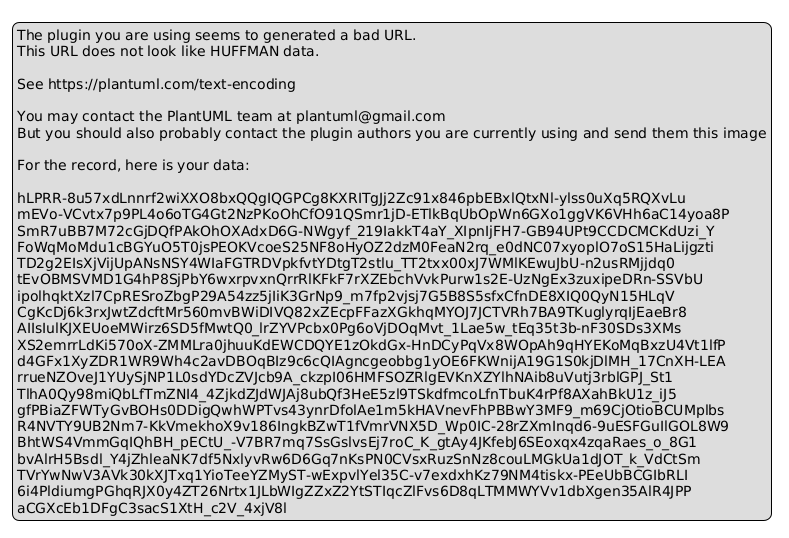
\includegraphics[width=\linewidth]{diagrams/deployment.png}
  \caption{UML Deployment diagram -- BrewLite trên Render (Production)}
  \label{fig:deployment}
\end{figure}

\subsubsection{Mô tả các node và ranh giới}

\paragraph{Local (docker-compose)}
Ba service chạy trên máy phát triển:
\begin{itemize}
  \item \texttt{brewlite-web} -- Next.js :3000, kết nối API qua \texttt{NEXT\_PUBLIC\_API\_URL=http://localhost:3001}.
  \item \texttt{brewlite-api} -- NestJS :3001, kết nối DB qua \texttt{DATABASE\_URL}.
  \item \texttt{brewlite-db} -- PostgreSQL 16 :5432, volume \texttt{pgdata}, healthcheck \texttt{pg\_isready}.
\end{itemize}

\paragraph{CI (GitHub Actions)}
Runner \texttt{ubuntu-latest} thực hiện: install $\to$ lint $\to$ test $\to$ build.
Sau khi pipeline pass, trigger Render Deploy Hook qua \texttt{curl} để deploy lên Production.

\paragraph{Production (Render)}
\begin{itemize}
  \item \textbf{Render CDN / Edge}: tiếp nhận HTTPS :443 từ người dùng, cấp TLS tự động (Let's Encrypt).
  \item \textbf{brewlite-web} (Render Web Service, Node.js 20): phục vụ Next.js, PORT=3000.
    Health check: \texttt{GET /menu}.
    Biến môi trường: \texttt{NEXT\_PUBLIC\_API\_URL}, \texttt{PORT}, \texttt{NEXT\_PUBLIC\_APP\_URL}.
  \item \textbf{brewlite-api} (Render Web Service, Node.js 20): NestJS API, PORT=3001.
    Health check: \texttt{GET /health} (implement ở Task 5.2).
    Biến môi trường: \texttt{DATABASE\_URL} (Render Internal URL), \texttt{JWT\_SECRET},
    \texttt{JWT\_EXPIRES\_IN}, \texttt{FRONTEND\_URL}, \texttt{NODE\_ENV=production},
    \texttt{ADMIN\_EMAIL}, \texttt{ADMIN\_PASSWORD}.
  \item \textbf{brewlite-db} (Render Managed PostgreSQL): kết nối qua Internal URL \texttt{:5432},
    persistent volume, không exposed ra internet.
\end{itemize}

Mọi secret lưu trong Render Environment Variables,
\textbf{không} xuất hiện trong repository hoặc log CI.

\subsubsection{Truy vết}

Mỗi node trong deployment diagram truy vết được tới thành phần trong kiến trúc (Task 3.1)
và thư mục mã nguồn:

\begin{center}
\begin{tabular}{lll}
\toprule
\textbf{Node (Deployment)} & \textbf{Kiến trúc (Task 3.1)} & \textbf{Mã nguồn} \\
\midrule
brewlite-web & Frontend Next.js (C4 Container) & \texttt{apps/web/} \\
brewlite-api & Backend NestJS (C4 Container) & \texttt{apps/api/} \\
brewlite-db  & PostgreSQL + TypeORM (C4 Container) & Migration trong \texttt{apps/api/src/migrations/} \\
GitHub Actions Runner & CI Pipeline & \texttt{.github/workflows/} \\
\bottomrule
\end{tabular}
\end{center}
